\section*{Linear Regression}
$y_i = \beta_1 x_{i1}+...+\beta_p x_{ip} + \epsilon_i$ (note: $x_{i1}\equiv 1$, so $\beta_1$ is intercept) where $\epsilon_1,...,\epsilon_n$ independent, $E(\epsilon_1)=0, \text{Var} (\epsilon_i)=\sigma^2$ (homoscedasticity)

\textbf{LSE:} $\hat \beta = \text{argmin}_\beta ||Y-Xb||_2^2 = (X^\top X)^{-1}X^\top Y \sim \mathcal{N}_p(\beta, \sigma^2 (X^\top X)^{-1})$ \\
$\hat \sigma^2 \approx \frac 1 {n-p}RSS$
also if error Gaussian then: $\hat Y \sim \mathcal{N}_n(X\beta, \sigma^2 P)$, error\\
$e \sim \mathcal{N}_n(0, \sigma^2(I-P))$,
$\hat \sigma^2 \sim {\sigma^2 }/{(n-p)}\cdot X_{n-p}$
where $P=X(X^\top X)^{-1}X^\top $

\textbf{Categorical Variables:} 
For two levels:$y_i = \beta_1 x_{i1}+...+\beta_p x_{ip} + \lambda d_{is} + \epsilon_i$ 
so if $i$ is in category, then $d_{is}=1$ else $d_{is}=0$. This acts as a different intercept ($E(y_i)-E(y_j)=\lambda$). If more categories, add more dummy variables.

\textbf{Interaction:} dummy can also influence slope: add term $\delta d_i x_i$, can influence interaction between predictors: add term $\delta x_{i2} x_{i3}$, can influence other categorical variable: add term $\delta d_{i1}d_{i2}$.

\subsection*{Measuring Goodness of Fit}
$H_0: y = X\beta + \epsilon$ with $\beta_j=0$
$H_A: y = X\beta + \epsilon$ with $\beta_j\neq 0$\\
Under $H_0: \frac{\hat \beta_j - (E[\hat \beta_j]=0)}{\sqrt{\sigma^2(X^\top X)^{-1}_{jj}}} \sim \mathcal{N}(0,1)$
t-statistic: $\frac{\hat \beta_j}{\sqrt{\hat \sigma^2 (X^\top X)^{-1}_{jj}}} \sim t_{n-p}$
\textbf{P-Value:} P(obs. a value of the test stat. that is as extreme or more extreme than the one we saw if $H_0$ is true).
If $< \alpha$ then reject $H_0$.
% Too lazy to draw this in LaTeX ;)
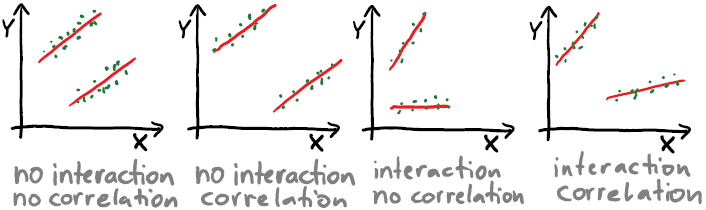
\includegraphics[width=0.7\linewidth]{interaction.PNG}

\begin{codebox}{r}{Linear Regression}
fit <- lm(y~x1+x2) # Fit only x1 and x2 (so p=3)
predict(fit, pred.data.frame)
# Manual fit
X <- cbind(1, x1, x2) # p = 3
XtX.inv <- solve(t(X) %*% X)
beta.hat <- XtX.inv %*% t(X.int) %*% y
res <- y - X.int %*% beta.hat # Residuals
RSE <- sqrt(sum(res^2)/(n-p)) # Residual std. error. Est. of the sd of the noise in the linear model
se.x1 <- RSE * sqrt(XtX.inv[2, 2]) # Std. error of x1
t.val.x1 <- beta.hat[2] / se.x1 # T value of x1
p.val.x1 <- 2*pt(abs(t.val.x1), df=n-p, lower=F)
# R squared: proportion of Var(y) that is explained by the fitted linear model.
RSE <- sqrt(sum(residuals(fit)^2)/(n-p))
RSS <- sum(res^2) # Residual sum of squares
TSS <- sum((y - mean(y))^2) # Total sum of squares
R.sq <- 1 - RSS / TSS
AdjR2 <- 1 - (RSS/(n-p))/(TSS/(n-1))
# Alternative t-value
coef <- summary(fit1)$coefficients
t1 <- coef["x1","Estimate"]/coef["x1","Std. Error"]
# Finding p-values
fit.smaller <- lm(y ~ x1)
anova(fit.smaller, fit, fit.all)
# Overall F-Test
fit.empty <- lm(y ~ 1, data=...) # Empty model
anova(fit.empty, fit) # Compare models
# Alternative F-test
Ftest <- summary(fit)$fstatistic
pval <- 1 - pf(Ftest[1], df1=Ftest[2], df2=Ftest[3])
# Categ. var. by hand & LOOCV
a1 <- (levels(shelveloc)[2]==shelveloc)*1
lcv<-mean((residuals(fit)/(1-lm.influence(fit)$h))^2)
\end{codebox}

\textbf{R Diagnostic plots: } \#1 Tukey-Anscombe Plot the points follow the line, else $E(\epsilon)=0$ violated. \#2 Q-Q Plot should follow line, else error not Gaussian (still all fine). \#3 Scale-Location: should be flat, else $\text{Var}(\epsilon_i)=\sigma^2$ violated (p-values wrong). \#4/\#5 Cook distance: shows if some data points have a larger impact on the fit than others (outliers). Note: cannot detect if the residuals are correlated with these plots!